\chapter{Reitinhaku}

Reitinhaku on keskeinen algoritmiikan ongelma, jossa haluamme
löytää parhaan reitin paikasta $a$ paikkaan $b$.
Esimerkiksi voimme haluta etsiä nopeimman tavan
matkustaa kotoa yliopistolle
tai halvimman lentoyhteyden kaupungista $a$
kaupunkiin $b$.
Verkkojen kielellä sanomme, että tavoitteemme on löytää \emph{lyhin polku}
solmusta $a$ solmuun $b$.

Jos verkon kaarilla ei ole painoja,
voimme löytää lyhimmät polut helposti leveyshaun avulla,
kuten olemme tehneet edellisessä luvussa.
Tässä luvussa kuitenkin keskitymme tilanteeseen,
jossa verkon kaarilla on painot.
Tässä tilanteessa tarvitsemme kehittyneempiä algoritmeja
lyhimpien polkujen löytämiseen.

Tutustumme kolmeen keskeiseen reitinhakumenetelmään:

\begin{itemize}
\item \textbf{Bellman–Fordin algoritmi} etsii lyhimmät polut
lähtösolmusta kaikkiin muihin solmuihin ajassa $O(nm)$.
\item \textbf{Dijkstran algoritmi} etsii lyhimmät polut
lähtösolmusta kaikkiin muihin solmuihin \emph{tehokkaammin} ajassa $O(m \log n)$
olettaen, että verkossa ei ole negatiivisen painoisia kaaria.
\item \textbf{Floyd–Warshallin algoritmi} etsii lyhimmät polut
\emph{kaikkien} verkon solmuparien välillä ajassa $O(n^3)$.
\end{itemize}

\section{Bellman–Fordin algoritmi}

Bellman–Fordin algoritmi laskee jokaiselle verkon solmulle,
kuinka pitkä on lyhin polku lähtösolmusta $x$ solmuun.
Algoritmi pitää yllä verkon solmuille arvioita,
mikä on etäisyys solmusta $x$ kyseiseen solmuun.
Aluksi etäisyys lähtösolmuun on 0 ja etäisyys kaikkiin muihin
solmuihin on $\infty$ (ääretön).
Sitten algoritmi alkaa parantaa etäisyyksiä
hyödyntämällä verkon kaaria.

Algoritmi muodostuu $n-1$ kierroksesta, joista jokainen käy läpi
kaikki verkon kaaret.
Jokaisen kaaren $a \rightarrow b$ kohdalla algoritmi tarkastaa,
voiko kaaren avulla parantaa etäisyyttä solmusta $x$ solmuun $b$
kulkemalla solmun $a$ kautta.
Jos näin on, algoritmi merkitsee uuden etäisyyden muistiin.
Algoritmin päätteeksi jokaisen solmun etäisyys on sama kuin
lyhimmän polun pituus solmusta $x$ kyseiseen solmuun.

\begin{figure}
\center
\begin{center}
\begin{tikzpicture}[scale=0.7,label distance=-1.5mm]
\small
\newcommand\verkko[6]{
\node[draw, circle] (1) at (0,-1) {$1$};
\node[draw, circle] (2) at (2,0) {$2$};
\node[draw, circle] (3) at (2,-2) {$3$};
\node[draw, circle] (4) at (4,0) {$4$};
\node[draw, circle] (5) at (4,-2) {$5$};
\path[draw,thick,->] (1) -- node[font=\small,label=above:8] {} (2);
\path[draw,thick,->] (1) -- node[font=\small,label=below:2] {} (3);
\path[draw,thick,->] (3) -- node[font=\small,label=right:4] {} (2);
\path[draw,thick,->] (2) -- node[font=\small,label=above:5] {} (4);
\path[draw,thick,->] (3) -- node[font=\small,label=below:7] {} (5);
\path[draw,thick,->] (5) -- node[font=\small,label=right:3] {} (4);
\node[color=red] at (0,-0.25) {$#2$};
\node[color=red] at (2,0.75) {$#3$};
\node[color=red] at (2,-2.75) {$#4$};
\node[color=red] at (4,0.75) {$#5$};
\node[color=red] at (4,-2.75) {$#6$};
\node at (2,-3.5) {vaihe #1};
}
\begin{scope}
\verkko{1}{0}{\infty}{\infty}{\infty}{\infty}
%\path[draw=red,thick,->,line width=2pt] (1) -- (2);
\end{scope}
\begin{scope}[xshift=6.5cm]
\verkko{2}{0}{8}{\infty}{\infty}{\infty}
\path[draw=red,thick,->,line width=2pt] (1) -- (2);
\end{scope}
\begin{scope}[xshift=13cm]
\verkko{3}{0}{8}{2}{\infty}{\infty}
\path[draw=red,thick,->,line width=2pt] (1) -- (3);
\end{scope}
\begin{scope}[yshift=-5.5cm]
\verkko{4}{0}{8}{2}{13}{\infty}
\path[draw=red,thick,->,line width=2pt] (2) -- (4);
\end{scope}
\begin{scope}[yshift=-5.5cm,xshift=6.5cm]
\verkko{5}{0}{6}{2}{13}{\infty}
\path[draw=red,thick,->,line width=2pt] (3) -- (2);
\end{scope}
\begin{scope}[yshift=-5.5cm,xshift=13cm]
\verkko{6}{0}{6}{2}{13}{9}
\path[draw=red,thick,->,line width=2pt] (3) -- (5);
\end{scope}
\begin{scope}[yshift=-11cm]
\verkko{7}{0}{6}{2}{12}{9}
\path[draw=red,thick,->,line width=2pt] (5) -- (4);
\end{scope}
\begin{scope}[yshift=-11cm,xshift=6.5cm]
\verkko{8}{0}{6}{2}{11}{9}
\path[draw=red,thick,->,line width=2pt] (2) -- (4);
\end{scope}
\end{tikzpicture}
\end{center}
\caption{Esimerkki Bellman–Fordin algoritmin toiminnasta.}
\label{fig:belfor}
\end{figure}

Kuva \ref{fig:belfor} näyttää esimerkin Bellman–Fordin algoritmin toiminnasta.
Tässä lähtösolmuna on solmu 1, ja haluamme selvittää siitä
lyhimmät polut muihin solmuihin.
Jokaisen solmun vieressä on ilmoitettu sen etäisyysarvio:
alussa etäisyys solmuun 1 on 0 ja etäisyys kaikkiin muihin solmuihin on ääretön.

Jokainen etäisyyden muutos näkyy kuvassa omana vaiheenaan.
Esimerkiksi ensimmäinen muutos on,
että saamme parannettua etäisyyttä solmuun 2,
koska voimme kulkea kaarta $1 \rightarrow 2$.
Tässä tapauksessa vanha etäisyys on $\infty$ ja uudeksi
etäisyydeksi tulee $8$.
Tässä esimerkissä vaiheiden 2--7 muutokset tapahtuvat
kierroksella 1 ja vaiheen 8 muutos tapahtuu kierroksella 2.
Tämän jälkeen kaikki etäisyydet ovat lopullisia,
eikä niihin tule enää muutoksia myöhemmillä kierroksilla.

Kuvasta voimme nähdä esimerkiksi,
että lyhin polku solmusta 1 solmuun 4 on painoltaan 11.
Tämä vastaa polkua $1 \rightarrow 3 \rightarrow 2 \rightarrow 4$.

\subsection{Analyysi}

Bellman–Fordin algoritmi muodostuu $n-1$ kierroksesta,
joista jokainen käy läpi verkon $m$ kaarta,
joten on helppoa nähdä, että algoritmi toimii ajassa $O(nm)$.
Mutta miksi on varmaa, että $n-1$ kierroksen jälkeen olemme
määrittäneet kaikki lyhimmät polut?

Ensimmäinen havainto on,
että $n$ solmun verkossa jokainen lyhin polku voi
sisältää enintään $n-1$ kaarta.
Jos polkuun kuuluisi $n$ tai enemmän kaaria,
jokin solmu esiintyisi polulla monta kertaa.
Tämä ei ole kuitenkaan mahdollista,
koska ei olisi järkeä kulkea monta kertaa saman solmun kautta,
kun haluamme saada aikaan lyhimmän polun.

Toinen havainto on, että jos lyhin polku solmusta $s_1$ solmuun $s_k$ on
$s_1 \rightarrow s_2 \rightarrow \dots \rightarrow s_k$,
niin myös lyhin polku solmusta $s_1$ solmuun $s_2$ on $s_1 \rightarrow s_2$,
lyhin polku solmusta $s_1$ solmuun $s_3$ on $s_1 \rightarrow s_2 \rightarrow s_3$, jne.,
eli jokainen polun alkuosa on myös lyhin polku vastaavaan solmuun.
Jos näin ei olisi, voisimme parantaa lyhintä polkua solmusta $s_1$ solmuun $s_k$
parantamalla jotain polun alkuosaa.

Tarkastellaan nyt, mitä tapahtuu algoritmin kierroksissa.
Ensimmäisen kierroksen jälkeen olemme löytäneet lyhimmät polut,
joissa on yksi kaari.
Toisen kierroksen jälkeen olemme löytäneet lyhimmät polut,
joissa on kaksi kaarta.
Sama jatkuu, kunnes $n-1$ kierroksen jälkeen olemme löytäneet
lyhimmät polut, joissa on $n-1$ kaarta.
Koska missään lyhimmässä polussa ei voi olla enempää kaaria,
olemme löytäneet kaikki lyhimmät polut.

\begin{figure}
\center
\begin{center}
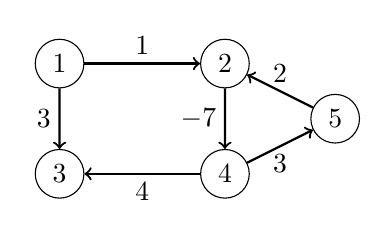
\begin{tikzpicture}[scale=0.7,label distance=-1.5mm]
\node[draw, circle] (1) at (1,3) {$1$};
\node[draw, circle] (2) at (4,3) {$2$};
\node[draw, circle] (3) at (1,1) {$3$};
\node[draw, circle] (4) at (4,1) {$4$};
\node[draw, circle] (5) at (6,2) {$5$};

\path[draw,thick,->] (1) -- node[font=\small,label=above:1] {} (2);
\path[draw,thick,->] (1) -- node[font=\small,label=left:3] {} (3);
\path[draw,thick,<-] (3) -- node[font=\small,label=below:4] {} (4);
\path[draw,thick,->] (2) -- node[font=\small,label=left:$-7$] {} (4);
\path[draw,thick,<-] (2) -- node[font=\small,label=above:2] {} (5);
\path[draw,thick,->] (4) -- node[font=\small,label=below:3] {} (5);
\end{tikzpicture}
\end{center}
\caption{Negatiivinen sykli $2 \rightarrow 4 \rightarrow 5 \rightarrow 2$,
jonka avulla voimme lyhentää polkuja loputtomasti.}
\label{fig:belsyk}
\end{figure}

Huomaa, että Bellman–Fordin algoritmi ei toimi järkevästi,
jos verkossa on \emph{negatiivinen sykli}
eli sykli, jonka kokonaispituus on negatiivinen.
Esimerkki tästä on kuvan \ref{fig:belsyk} verkossa oleva sykli
$2 \rightarrow 4 \rightarrow 5 \rightarrow 2$, jonka paino on $-2$.
Negatiivisen syklin avulla voimme lyhentää polkuja loputtomasti kulkemalla
sykliä uudestaan ja uudestaan, eikä lyhimmän polun pituudella ole alarajaa.
Voimme havaita negatiivisen syklin olemassaolon suorittamalla
algoritmia $n$ kierrosta tavallisen $n-1$ sijaan.
Jos viimeisellä kierroksella jokin etäisyys pienenee,
verkossa on negatiivien sykli.

\subsection{Toteutus}

Bellman–Fordin algoritmi on kätevää toteuttaa käyttäen verkon
kaarilista\-esitystä. Meillä on siis lista

\begin{code}
ArrayList<Kaari> kaaret = new ArrayList<>();
\end{code}

jonka jokainen alkio vastaa yhtä kaarta.
Lisäksi määrittelemme taulukon

\begin{code}
int[] etaisyys = new int[n+1];
\end{code}

joka pitää kirjaa solmujen etäisyyksistä.
Alustamme taulukon näin:

\begin{code}
for (int i = 1; i <= n; i++) {
    etaisyys[i] = 1e9;
}
etaisyys[x] = 0;
\end{code}

Koska Javassa ei ole käsitettä ''ääretön'', käytämme sen sijasta
suurta lukua $10^9$, eli oletamme, että kaikki etäisyydet
ovat pienempiä kuin $10^9$.
Jos etäisyydet voivat olla suurempia, tätä lukua täytyy muuttaa.

Tämän jälkeen voimme toteuttaa algoritmin näin:

\begin{code}
for (int i = 1; i <= n-1; i++) {
    for (Kaari kaari : kaaret) {
        int vanha = etaisyys[kaari.loppu];
        int uusi = etaisyys[kaari.alku]+kaari.paino;
        etaisyys[kaari.loppu] = Math.min(vanha, uusi);
    }
}
\end{code}

Entä jos haluamme myös saada selville,
mitä kaaria on lyhimmällä polulla solmusta $x$ solmuun $y$?
Tällöin voimme laajentaa algoritmia niin,
että se pitää yllä myös taulukkoa

\begin{code}
int[] edellinen = new int[n+1];
\end{code}

joka kertoo jokaiselle solmulle, mikä on sitä edeltävä
solmu lyhimmällä polulla.
Päivitämme tätä taulukkoa aina silloin,
kun jokin etäisyys pienenee.
Taulukon avulla voimme muodostaa käänteisesti
lyhimmän polun mihin tahansa solmuun.

\section{Dijsktran algoritmi}

\section{Floyd-Warshallin algoritmi}
